
\section{Deliverable 2: MNIST Dataset Cutom CNN Loss Plot for Training and Validation Data}

\begin{solve}
    

    \begin{figure}[H]
        \centering
        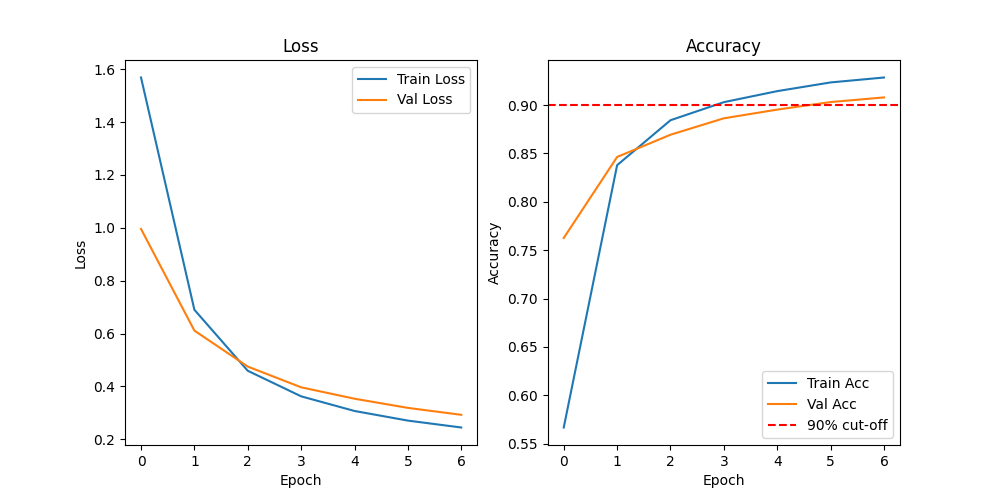
\includegraphics[width=0.9\textwidth]{/Users/vashisth/Documents/GitHub/Intro_DL/IDL_HW3/code/deliverable1-2/train-loss-curve-del1-2.png}
        \caption{Loss Accuracy Plot for Deliverable 1-2}
    \end{figure}

\begin{lstlisting}[language=python, title=Train Logs, basicstyle=\scriptsize](deep_learning) vashisth@Vashisths-MacBook-Pro deliverable1-2 % python3 train.py 
LOAD DATASET: TRAIN 60000 | TEST: 10000
Epoch 1  | Train Loss: 1.5684 | Train Acc: 0.5666 | Val Loss: 0.9956 | Val Acc: 0.7626
Epoch 2  | Train Loss: 0.6898 | Train Acc: 0.8379 | Val Loss: 0.6110 | Val Acc: 0.8464
Epoch 3  | Train Loss: 0.4591 | Train Acc: 0.8844 | Val Loss: 0.4750 | Val Acc: 0.8694
Epoch 4  | Train Loss: 0.3624 | Train Acc: 0.9031 | Val Loss: 0.3965 | Val Acc: 0.8864
Epoch 5  | Train Loss: 0.3070 | Train Acc: 0.9145 | Val Loss: 0.3534 | Val Acc: 0.8954
Epoch 6  | Train Loss: 0.2706 | Train Acc: 0.9235 | Val Loss: 0.3187 | Val Acc: 0.9032
Epoch 7  | Train Loss: 0.2445 | Train Acc: 0.9286 | Val Loss: 0.2925 | Val Acc: 0.9080
Training time: 1516.1303s
\end{lstlisting}

\end{solve}